\documentclass[border=10pt]{standalone}
\usepackage{tikz}
\usetikzlibrary{positioning, arrows.meta, calc, fit, backgrounds}

\definecolor{partI}{RGB}{66,133,244}
\definecolor{partII}{RGB}{234,67,53}
\definecolor{partIII}{RGB}{251,188,4}
\definecolor{partIV}{RGB}{52,168,83}
\definecolor{partV}{RGB}{153,102,204}

\begin{document}
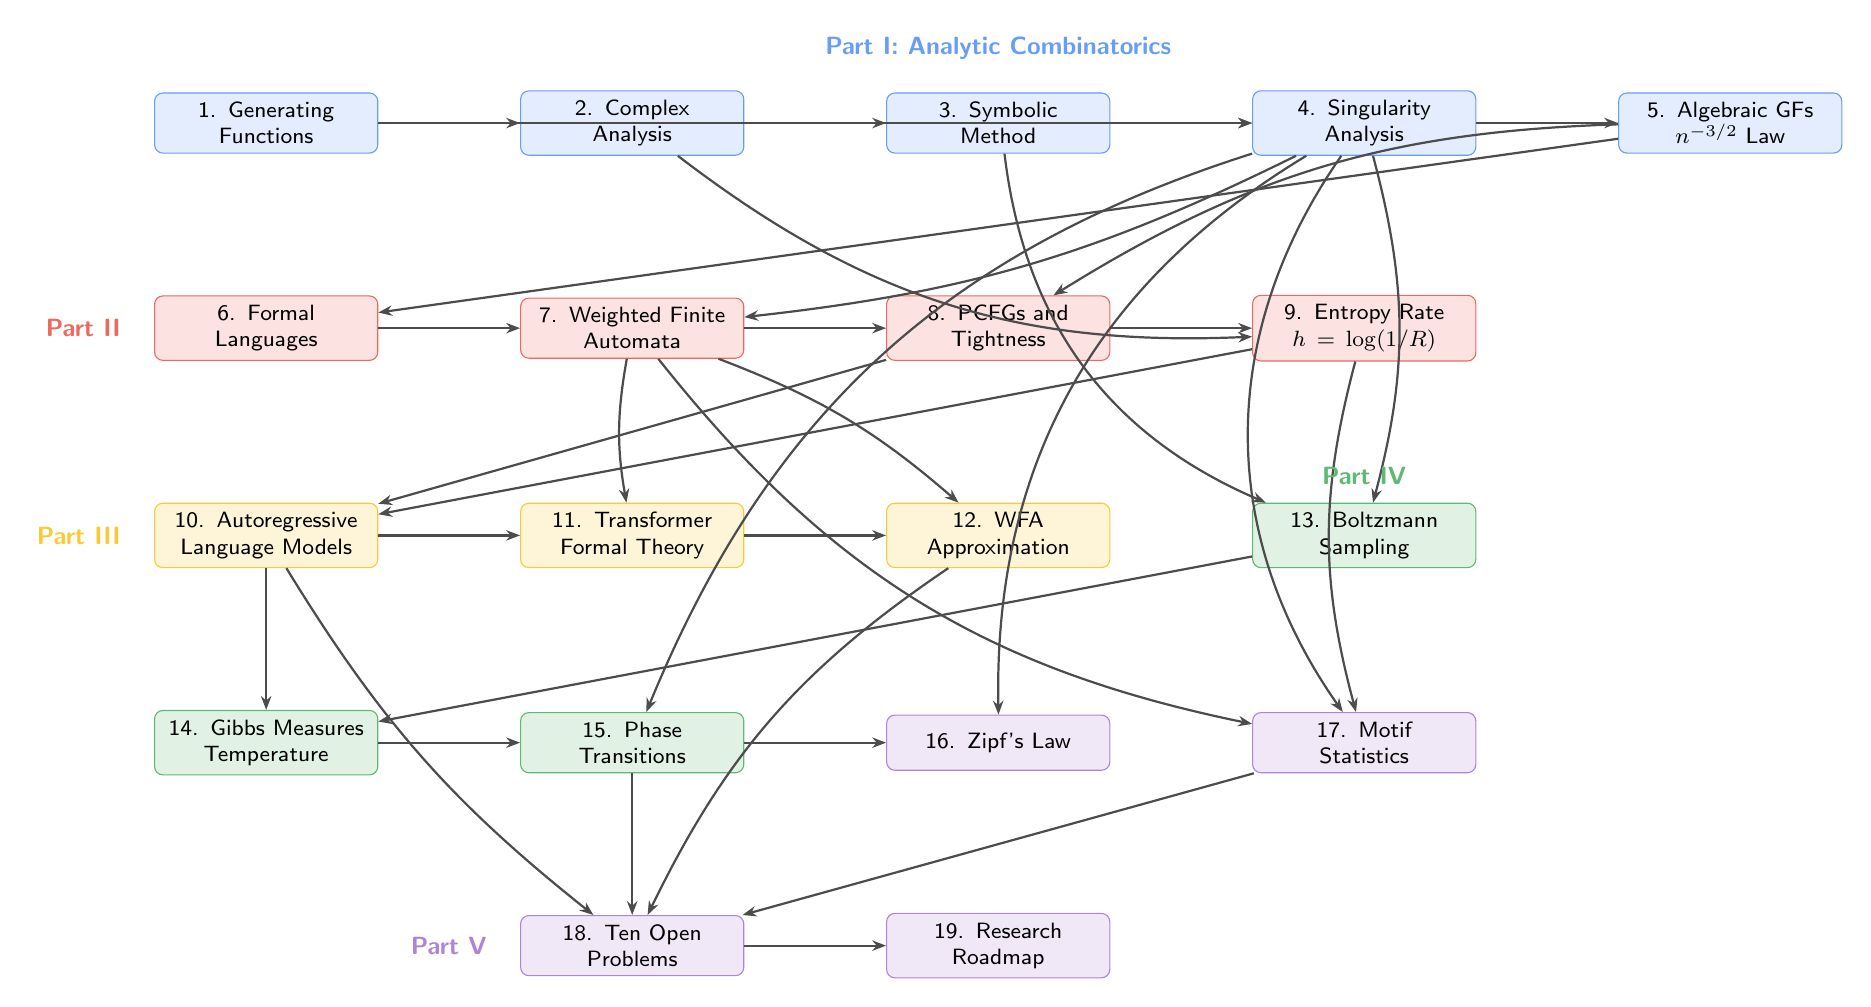
\begin{tikzpicture}[
    node distance=1.2cm and 1.8cm,
    ch/.style={
        rectangle, rounded corners=3pt, draw=#1!80, fill=#1!15,
        minimum width=2.8cm, minimum height=0.7cm,
        font=\footnotesize\sffamily, align=center, text width=2.6cm
    },
    essential/.style={-{Stealth[length=5pt]}, thick, draw=black!70},
    optional/.style={-{Stealth[length=4pt]}, dashed, thin, draw=black!30},
    partlabel/.style={font=\small\sffamily\bfseries, text=#1!80}
]

% Part I (blue) — row 1
\node[ch=partI] (ch1) {1. Generating\\Functions};
\node[ch=partI, right=of ch1] (ch2) {2. Complex\\Analysis};
\node[ch=partI, right=of ch2] (ch3) {3. Symbolic\\Method};
\node[ch=partI, right=of ch3] (ch4) {4. Singularity\\Analysis};
\node[ch=partI, right=of ch4] (ch5) {5. Algebraic GFs\\$n^{-3/2}$ Law};

% Part II (red) — row 2
\node[ch=partII, below=1.8cm of ch1] (ch6) {6. Formal\\Languages};
\node[ch=partII, right=of ch6] (ch7) {7. Weighted Finite\\Automata};
\node[ch=partII, right=of ch7] (ch8) {8. PCFGs and\\Tightness};
\node[ch=partII, right=of ch8] (ch9) {9. Entropy Rate\\$h = \log(1/R)$};

% Part III (yellow) — row 3
\node[ch=partIII, below=1.8cm of ch6] (ch10) {10. Autoregressive\\Language Models};
\node[ch=partIII, right=of ch10] (ch11) {11. Transformer\\Formal Theory};
\node[ch=partIII, right=of ch11] (ch12) {12. WFA\\Approximation};

% Part IV (green) — row 3, right side
\node[ch=partIV, right=of ch12] (ch13) {13. Boltzmann\\Sampling};

% Part IV continued — row 4
\node[ch=partIV, below=1.8cm of ch10] (ch14) {14. Gibbs Measures\\Temperature};
\node[ch=partIV, right=of ch14] (ch15) {15. Phase\\Transitions};

% Part V (purple) — row 4, continued
\node[ch=partV, right=of ch15] (ch16) {16. Zipf's Law};
\node[ch=partV, right=of ch16] (ch17) {17. Motif\\Statistics};

% Row 5
\node[ch=partV, below=1.8cm of ch15] (ch18) {18. Ten Open\\Problems};
\node[ch=partV, right=of ch18] (ch19) {19. Research\\Roadmap};

% === Essential dependencies (solid arrows) ===
% Part I chain
\draw[essential] (ch1) -- (ch2);
\draw[essential] (ch1) -- (ch3);
\draw[essential] (ch2) -- (ch4);
\draw[essential] (ch3) -- (ch4);
\draw[essential] (ch4) -- (ch5);

% Part I -> Part II
\draw[essential] (ch5) -- (ch6);
\draw[essential] (ch4) to[bend left=10] (ch7);
\draw[essential] (ch6) -- (ch7);
\draw[essential] (ch5) to[bend right=15] (ch8);
\draw[essential] (ch7) -- (ch8);
\draw[essential] (ch2) to[bend right=20] (ch9);
\draw[essential] (ch8) -- (ch9);

% Part II -> Part III
\draw[essential] (ch8) -- (ch10);
\draw[essential] (ch9) -- (ch10);
\draw[essential] (ch7) to[bend right=10] (ch11);
\draw[essential] (ch10) -- (ch11);
\draw[essential] (ch7) to[bend left=10] (ch12);
\draw[essential] (ch11) -- (ch12);

% Part I -> Part IV
\draw[essential] (ch3) to[bend right=30] (ch13);
\draw[essential] (ch4) to[bend left=15] (ch13);

% Part III/IV connections
\draw[essential] (ch10) -- (ch14);
\draw[essential] (ch13) -- (ch14);
\draw[essential] (ch4) to[bend right=25] (ch15);
\draw[essential] (ch14) -- (ch15);

% Part V
\draw[essential] (ch4) to[bend right=30] (ch16);
\draw[essential] (ch15) -- (ch16);
\draw[essential] (ch4) to[bend right=35] (ch17);
\draw[essential] (ch7) to[bend right=20] (ch17);
\draw[essential] (ch9) to[bend right=15] (ch17);

% Ch18 synthesis
\draw[essential] (ch10) to[bend right=10] (ch18);
\draw[essential] (ch12) to[bend right=15] (ch18);
\draw[essential] (ch15) -- (ch18);
\draw[essential] (ch17) -- (ch18);

% Ch19
\draw[essential] (ch18) -- (ch19);

% === Part labels ===
\node[partlabel=partI, above=0.3cm of ch3] {Part I: Analytic Combinatorics};
\node[partlabel=partII, left=0.3cm of ch6, anchor=east] {Part II};
\node[partlabel=partIII, left=0.3cm of ch10, anchor=east] {Part III};
\node[partlabel=partIV, above=0.1cm of ch13, anchor=south] {Part IV};
\node[partlabel=partV, left=0.3cm of ch18, anchor=east] {Part V};

\end{tikzpicture}
\end{document}
